% !TeX root = ../Main.tex
\section{Zahlen und Vektoren}
	\begin{multicols}{2}
			\begin{definition}[Eigenschaften der Norm]\hfill\\
				Eine Norm hat folgende Eigenschaften:
				\begin{enumerate}
					\item Definitheit: $\norm{x} \geq 0, \quad \norm{x} = 0 \Rightarrow x = 0$
					\item Positive Homogenität: $\norm{\alpha x} = \abs{\alpha} \norm{x}$
					\item Dreiecksungleichung: $\norm{x + y} \leq \norm{x} + \norm{y}$
				\end{enumerate}
			\end{definition}
			\begin{theorem}[Archimedisches Prinzip]
				Zu jeder Zahl $0 < b \in \mathbb{R}$ gibt es ein $n \in \mathbb{N}$ mit $b < n$
			\end{theorem}
			\begin{theorem}[Young Ungleichung]
				Für $x,y \in \mathbb{R}, \varepsilon > 0$ gilt
				\begin{equation*}
					2 \abs{x \cdot y} \leq \varepsilon x^2 + \frac{1}{\varepsilon} y^2
				\end{equation*}
			\end{theorem}
			\begin{theorem}[Dreiecksungleichungen]
				Es gilt: 
				\begin{align*}
					\abs{\sum\limits_{i=1}^{n} x_i} &\leq \sum\limits_{i=1}^{n} \abs{x_i} \\
					\abs{\prod\limits_{i=1}^{n} x_i} &= \prod\limits_{i=1}^{n} \abs{x_i} \\
					\abs{x \pm y} &\geq \abs{\abs{x} - \abs{y}} 
				\end{align*}
			\end{theorem}
%		\subsection{Supremum und Infimum}
%			\begin{definition}
%				Eine Menge $A \subset \mathrm{R}$ heisst \highlight{nach oben beschränkt}, falls gilt
%				$$
%					\exists b \in \mathrm{R} \, \forall a \in A \, : \, a \leq b
%				$$
%				Jedes solche $b$ heisst \highlight{obere Schranke} für $A$.
%			\end{definition}
%			\begin{theorem}
%				Für jede Menge $A \subset \mathbb{R}$ gilt:
%				\begin{itemize}
%					\item $A$ nach oben beschränkt $\Rightarrow$ A hat \highlight{Supremum}
%					\item $A$ nach unten beschränkt $\Rightarrow$ A hat \highlight{Infimum}
%				\end{itemize}
%			\end{theorem}
			\begin{theorem}[Cauchy-Schwarz]
				\begin{equation*}
					\forall x,y \in \mathbb{R}^n \, : \, \abs{\dotp{x}{y}} \leq \norm{x} \cdot \norm{y}
				\end{equation*}
			\end{theorem}
		
%		\subsection{Ordnungsvollständigkeit von $\mathbb{R}$}
%			\begin{theorem}[Ordnungsvollständigkeit]
%				Zu je zwei nicht leeren Mengen $A, B \subset \mathbb{R} $ mit 
%				$$ \forall a \in A \, , b \in B \, : \, a \leq b $$
%				gibt es ein $c \in \mathbb{R}$, sodass gilt
%				$$ \forall a \in A \, , b \in B \, : \, a \leq c \leq b $$
%			\end{theorem}
		
		
	\end{multicols}
	\subsection{Komplexe Zahlen}
		\begin{multicols}{2}
			\begin{hint}[Kartesische Koordinaten]
				Zur Addition von komplexen Zahlen eignet sich vor allem die Darstellung in kartesischen Koordinaten: 
				$$ z = x + \imath \cdot y$$
				Bei der Division in kartesischen Koordinaten muss mit der konjugiert komplexen Zahl des Divisors erweitert werden. 
			\end{hint}
			\begin{hint}[Polarform]
				Zum Multiplizieren, Dividieren, Wurzelziehen ist die Polarform geeignet:
				$$ z = r \cdot (\cos \varphi + \imath \sin \varphi ) \overset{(Euler)}{=} r \cdot \emath^{\imath \cdot \varphi}$$
			\end{hint}
			\begin{hint}[Wurzeln]
				Die Gleichung $z^n = R \cdot \emath^{\imath \cdot \omega}$ hat folgende Lösungen:
				$$
				\sqrt[n]{R} \cdot \emath^{\imath \cdot \left(\tfrac{\omega}{n} + \tfrac{2 \pi k}{n} \right)} \quad \vert \quad k = 0, 1, 2, 3 \dots n - 1
				$$
			\end{hint}
			\begin{hint}[Mengen komplexer Zahlen]
				Mengen komplexer Zahlen lassen sich meist am einfachsten beschreiben, wenn der Realteil und der Imaginärteil getrennt betrachtet werden. So lassen sich auch komplexe Gleichungssysteme meist einfach lösen. 
				Eventuell kann auch die Darstellung in Polarform nützlich sein.
			\end{hint}
		\end{multicols}
		
	\subsection{Nullstellenberechnung}
		\begin{hint}[Hornerschema]\hfill\\
			\begin{center}
			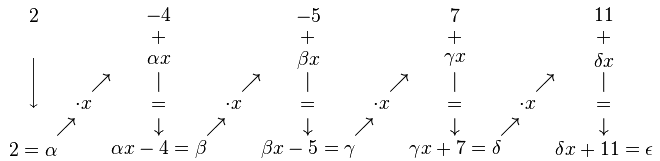
\includegraphics[scale=0.7]{./Images/Hornerschema.png}
			\end{center}
		\end{hint}